%%%%%%%%%%%%%%%%%%%%%%%%%%%%%%%%%%%%%%%%%%%%%%%%%%%%%%%%%%%%%%%%%%%%%%%%
% Plantilla TFG/TFM
% Escuela Politécnica Superior de la Universidad de Alicante
% Realizado por: Jose Manuel Requena Plens
% Contacto: info@jmrplens.com / Telegram:@jmrplens
%%%%%%%%%%%%%%%%%%%%%%%%%%%%%%%%%%%%%%%%%%%%%%%%%%%%%%%%%%%%%%%%%%%%%%%%

\chapter{Arrays de Antenas}
\label{arraysdeantenas}

\section{Introducción}

\par Un array o vector de antenas se basa en la agrupación de un cierto número de elementos individuales de antenas para conseguir que trabajen como una sola, mejorando así las prestaciones globales de esta e incluso llegar a obtener parámetros característicos que serían imposibles de conseguir con el trabajo de una sola antena.
\\
\par En cierto tipo de aplicaciones, necesitamos patrones de radiación o ganancias que antenas de un único elemento no nos pueden ofrecer, ya que los patrones de directividad de estos suelen ser anchos y muy poco directivos. Cuando se necesitan antenas con ganancias más elevadas o patrones de directividad estrechos y concentrados para, por ejemplo, radio enlaces, o patrones estrechos en un plano, pero muy extendidos en su perpendicular, como se hace necesario en aplicaciones de telefonía móvil donde se intenta concentrar el haz hacia las calles y las casas y evitar propagar la señal al cielo, se hace indispensable el uso de agrupaciones de antenas para modelar la radiación de la señal según nuestras especificaciones.
\\
\par Normalmente un array de antenas está formado por la agrupación del mismo tipo y modelo de antenas dispuestas en una geometría específica. Aunque esto no es estricto, y diferentes tipos de antenas pueden actuar como array para conseguir configuraciones más específicas o cuando otro tipo de limitaciones, como factores de diseño o económicos, no nos permiten usar el mismo tipo de antenas.
\\
\par Cuando se dispone de un array de antenas, lo común es que este se diseñe para que el campo electromagnético radiado total sea la suma de los campos individuales trabajando en forma de interferencia constructiva para el lóbulo principal, y en forma de interferencia destructiva para el resto del espacio, de forma que la máxima transferencia de potencia se centre en el lóbulo principal. Para conseguir un correcto funcionamiento de un array de antenas según las especificaciones marcadas para nuestra aplicación se deberán tener en cuenta una serie de factores clave en el diseño \cite{Valero2008}:

\begin{itemize}
\item \textbf{La configuración geométrica: }Se deberá conocer de antemano qué tipo de configuración geométrica se aplicará a la hora de distribuir los elementos individuales: Lineal, circular, rectangular, etc. Esta distribución es clave para la correcta aproximación a los parámetros finales deseados.

\item \textbf{Distancia entre elementos: }La distancia entre elementos  afectará a como los campos electromagnéticos interfieren entre si y estos son sumados en el campo lejano.

\item \textbf{La amplitud de excitación: }Una incorrecta intensidad de excitación a uno o varios de los elementos que conformen el array puede llevar a superposiciones indeseadas que deformen por completo el patrón de radiación de nuestra antena global.

\item \textbf{La fase de excitación: }La fase con la que se alimenta cada elemento individual es un factor clave para modelar el comportamiento global de la antena. Si se alimenta cada elemento siempre con la misma fase se obtendrá un patrón de radiación concreto y estático mientras que el hecho de variar la fase a cada elemento de forma individual hará que el patrón de radiación varíe según las necesidades. Esta variación de fase es normalmente llevada a cabo por ordenador y son también conocidos como \textit{Phased arrays}

\item \textbf{El patrón de radiación de cada elemento: }Para que un elemento llegue a interferir constructiva o destructivamente sobre la radiación de otro, es necesario que sus patrones lleguen a mezclarse físicamente, para ello, el patrón de radiación de cada elemento individual debe estar controlado para así poder predecir cual será el resultado de la antena global.
\end{itemize}

\section{Arrays lineales}
\par Para entender el funcionamiento analítico de las agrupaciones de antenas, se pondrá como ejemplo un array lineal de estas. Un array lineal consiste en un conjunto de antenas agrupadas a lo largo de una recta y conectadas en serie. El diagrama de radiación del array de antenas es el producto final de las interferencias constructivas y destructivas causadas por las radiaciones de los elementos individuales. Comenzaremos considerando una sola antena alimentada mediante una corriente $I_{n}$, donde $n$ identifica el número de la antena que compone el array, siendo 0 la primera antena y N-1 la última. Por lo tanto, la primera antena será alimentada por una corriente $I_{0}$ \citep{Cardama2002}.
\\
\par Esta antena poseerá una distribución de corrientes $J_{0}(\vec{r})$. Por lo tanto, si agrupamos un conjunto de $n$ antenas equiespaciadas una distancia $d$ a lo largo del eje $z$ (fig. \ref{fig:arraigo}), cada una excitada con su fasor de corriente, $I_{n}$, la distribución de corrientes del conjunto de antenas quedará como \cite{Cardama2002}:

\begin{figure}[h]
    \centering
        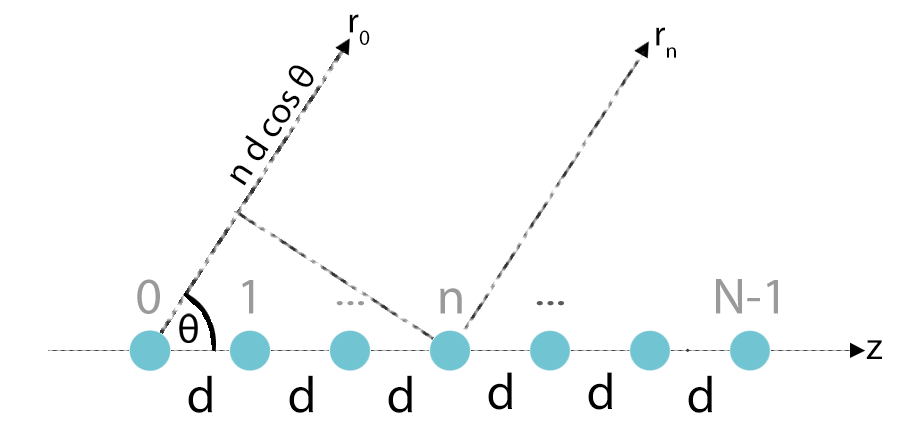
\includegraphics[width=0.65\textwidth]{archivos/array/array}
        \caption{Agrupación lineal de antenas sobre el eje Z}
        \label{fig:arraigo}
\end{figure}

\begin{equation}
	\vec{J}\left ( \vec{r} \right )=\sum_{n=0}^{N-1}I_{n}\vec{J}_{0}(r-nd\hat{z})
	\label{eq:distrib}
\end{equation}

\par Se puede expresar el sumatorio anterior como la convolución entre la corriente que alimenta un elemento básico del array, es decir, una antena simple, y un tren de deltas ponderadas con sus respectivos pesos $I_{n}$ \cite{Cardama2002}.

\begin{equation}
	\vec{J}\left ( \vec{r} \right )=\vec{J}_{0}\left ( \vec{r} \right ) \ast \sum_{n=0}^{N-1}I_{n}\delta (r-nd\hat{z})=\vec{J}_{0}\left ( \vec{r} \right )\ast I(n)
	\label{eq:conv}
\end{equation}

\par Sabiendo que el vector de radiación $\vec{N}\left ( \vec{r} \right )$, es la transformada de Fourier tridimensional de la distribución de corrientes $\vec{J}\left ( \vec{r} \right )$, se aplicará el teorema de convolución para calcularlo \cite{Cardama2002}.

\begin{equation}
	\vec{N}\left ( \vec{r} \right )=TF_{3D}\left [\vec{J}\left ( \vec{r} \right )  \right ]=\vec{N}_{0}\left ( \vec{r} \right )\cdot TF_{3D}\left [ I(n)   \right ]
	\label{eq:3d}
\end{equation}

\par Donde $\vec{N}_{0}\left ( \vec{r} \right )$ es el vector de radiación del elemento simple situado en el origen, cuando el fasor de alimentación toma el valor unidad. Dado que el fasor de corriente $I_{n}$  es separable, su $TF_{3D}$ consistirá en el producto de las transformadas en cada dirección \cite{Cardama2002}.


\begin{equation}
	TF_{3D}\left [ I(n)   \right ]= TF_{x}\left [ I(n)   \right ]\cdot TF_{y}\left [ I(n)   \right ]\cdot TF_{z}\left [ I(n)   \right ] = TF_{z}\left [ I(n)   \right ] = \sum_{n=0}^{N-1}I_{n} e^{j\omega _{z}n}
	\label{eq:direccional}
\end{equation}

\par Donde $\omega _{z}$ es la frecuencia digital en la dirección del eje $z$, que puede ser obtenida mediante el producto de la frecuencia espacial analógica $k_{z}$  por el periodo de muestreo en la dirección z, que equivale a la distancia de espaciación entre las antenas que componen el array, $d$ \cite{Cardama2002}. 

\begin{equation}
	\omega_{z} = k_{z}\cdot d = k d \cos {\theta } 
	\label{eq:frecdigital}
\end{equation}

\par Donde $\theta$ representa el ángulo cualquiera con respecto a la agrupación de antenas. Teniendo en cuenta que los fasores de alimentación $I_{n}$, presentan una fase progresiva entre cada par de antenas consecutivas que puede expresarse mediante \cite{Cardama2002}: 

\begin{equation}
	I_{n}=a_{n}e^{jn\alpha} 
	\label{eq:fasor}
\end{equation}

\par Donde $a_{n}$ son coeficientes, generalmente complejos, y que pueden tomar valores reales cuando la fase de alimentación sea progresiva, se podrá entonces
obtener el vector de radiación del conjunto de antenas \cite{Cardama2002}:

\begin{equation}
	\vec{N}\left ( \vec{r} \right )= \vec{N}_{0}\left ( \vec{r} \right )\sum_{n=0}^{N-1}a_{n}e^{jn(kd\cos\theta+\alpha)}
	\label{eq:vecrad}
\end{equation}

\par Para simplificar los cálculos, agruparemos el término $kd\cos\theta+\alpha$ en una sola variable, la cual representará la diferencia de fase entre las contribuciones en el campo lejano de dos antenas consecutivas \cite{Cardama2002}. 

\begin{equation}
	\Psi = kd\cos\theta+\alpha
	\label{eq:psi}
\end{equation}

\par Esta diferencia de fase es igual a la suma del desfase por diferencia de caminos $kd\cos\theta$, más la diferencia de fase que progresivamente ha ido alimentando cada antena $\alpha$. Quedando entonces el vector de radiación como \cite{Cardama2002}: 

\begin{equation}
	\vec{N}\left ( \vec{r} \right )= \vec{N}_{0}\left ( \vec{r} \right )\sum_{n=0}^{N-1}a_{n}e^{jn\Psi}
	\label{eq:vecrad2}
\end{equation}

\par Se puede observar cómo el vector de radiación consiste en el producto entre el vector de radiación de la primera antena básica $\vec{N}_{0}\left ( \vec{r} \right ) $ y un factor que tiene en cuenta la interferencia de las \textit{N} ondas generadas por cada antena. Este factor depende unicamente de la separación entre elementos, su alimentación y la frecuencia de trabajo, y se le denomina \textit{factor de agrupación} o \textit{factor de array} (\textit{FA}) \cite{Cardama2002}.

\begin{equation}
	FA(\Psi)=\sum_{n=0}^{N-1}a_{n}e^{jn\Psi}
	\label{eq:fa}
\end{equation}

\section{Factor de array}

\par Mediante el factor de array se puede obtener el patrón de radiación producido por cualquier array de antenas isotrópicas. Si las antenas que conforman el array no fuesen isotrópicos, se podrá obtener el campo radiado total multiplicando el factor de array por el campo radiado de un elemento único. Cada array tiene su propio factor de array. El factor de array, por lo general, queda en función del número de elementos, su disposición geométrica, sus magnitudes relativas, sus fases relativas, y la distancia entre los elementos \cite{Balanis2015}. 
\\
\par El factor de array presenta las siguientes propiedades \cite{Cardama2002}:

\begin{itemize}
\item \textbf{Periodicidad: }Se trata de una función periódica del ángulo $\Psi$ con periodo $2\pi$, tal que los coeficientes de su serie de Fourier son los coeficientes de la alimentación $a_{n}$. Gracias a esta propiedad se podrá realizar una sintetización de un patrón de radiación mediante el ajuste de los coeficientes de Fourier del factor de array de la agrupación concreta.

\item \textbf{Relación con la TF: }El factor de array puede ser definido ahora como la transformada de Fourier de la secuencia discreta de los coeficientes de la alimentación, $a_{n}$.

\item \textbf{Máximo del factor de array: }Si los coeficientes de la alimentación $a_{n}$ son reales y positivos, el máximo del factor de la agrupación se encuentra en el origen $\Psi=0$. Sabiendo que el máximo del diagrama de radiación se encuentra en la dirección en la que los máximos de cada antena se interfieren positivamente en el espacio, es decir, en fase, la cual corresponde a un desfase nulo ($\Psi=0$) en la interferencia cuando los coeficientes son reales y positivos.

\item \textbf{Margen visible: }Dado que el ángulo $\theta$ solo tomará valores reales entre 0 y $\pi$, se puede deducir el rango de valores de $\Psi$ para los que este fenómeno toma lugar:

\begin{equation}
	\Psi \in \left [ -kd+\alpha ,\; kd+\alpha \right ]
	\label{eq:dominio}
\end{equation}

\par Solamente el intervalo comprendido en (\ref{eq:dominio}) pertenece al diagrama de radiación, lo que se conoce como \textit{margen visible} (fig. \ref{margenvisible}). La longitud del margen visibles es de $2kd$ y está centrado en $\Psi=\alpha$, de forma que su tamaño es proporcional al espaciado de la agrupación, normalizado respecto a la longitud de onda y su posición en el eje $\Psi$ varía con la fase progresiva.

\item \textbf{Máximo del diagrama de radiación: }Cuando los coeficientes de la alimentación son reales y positivos y si el margen visible incluye el origen $\Psi=0$, el máximo del diagrama de radiación se encuentra en $\theta_{max}$. 

 \begin{equation}
	\theta_{max}=\arccos(-\frac{\alpha}{kd}),\ \ \left | \alpha \right |\leq kd
	\label{eq:radmax}
\end{equation}

\par Si se varía la fase de alimentación progresiva $\alpha$, sería posible controlar la dirección del máximo de radiación. Este es el principio de funcionamiento de los \textit{Phased arrays}, en las que la dirección del máximo se varía de forma electrónica mediante un control de la fase relativa progresiva de alimentación de los elementos individuales del array. 

\textbf{Periodicidad de los máximos: }Si el máximo de radiación se encuentra en $\Psi_{max}$ existirán máximos periódicos en los múltiplos enteros de $2\pi$. Cuando estos máximos se encuentran dentro del margen visible:

\begin{equation}
	kd+\alpha\geq 2\pi,\ \
-kd+\alpha\leq 2\pi  
\label{eq:maxdominio}
\end{equation}


\par Aparecerán múltiples máximos de radiación en el espacio real, denominados \textit{lóbulos de difracción} o \textit{grating lobes}. Este fenómeno suele darse cuando el espaciado es de una o más longitudes de onda.
\begin{figure}[h]
    \centering
        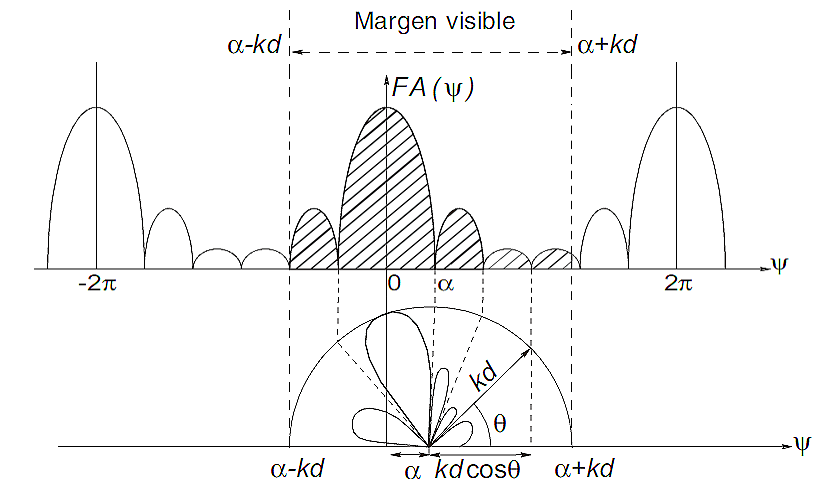
\includegraphics[width=0.62\textwidth]{archivos/array/margen}
        \caption{Margen visible. \cite{Cardama2002}}
        \label{fig:margenvisible}
\end{figure}

\end{itemize}



\newpage
\section{Influencia de los parámetros de diseño}
\par A continuación, se van a realizar un breve resumen sobre los principales efectos que producen sobre el patrón de radiación la modificación de los parámetros de diseño del array, tales como el número de elementos que lo componen, la distancia entre ellos, o el efecto que produciría un desfase relativo en su alimentación. Para la simulación de los efectos deseados se usará el Applet diseñado por Amanogawa para la simulación de arrays uniformes \cite{Amanogawa2019}.

\subsection{Número de elementos}
\par En primer lugar se comenzará variando el número de elementos que componen el array de dipolos uniformes. La configuración del array se basará en la adición de dipolos de longitud $\lambda/2$, alimentados con la misma fase relativa y separados a una distancia entre $\lambda/4$ y $\lambda$ para poder ver cómo la separación entre elementos también afecta a la forma inicial del patrón de radiación.
\\
\par En la tabla \ref{tab:numeroelementos} se puede observar cómo, dado un espacio constante y un aumento del número de elementos del array, la directividad del patrón de radiación va aumentando, y con ello, el número de lóbulos laterales. Se ha de llegar a un compromiso entre la directividad que se desea conseguir en el patrón de directividad final frente al número de lóbulos laterales y la intensidad de estos, a la hora de diseñar un array lineal.


\begin{table}[h]
\centering
\begin{tabular}{ccc}
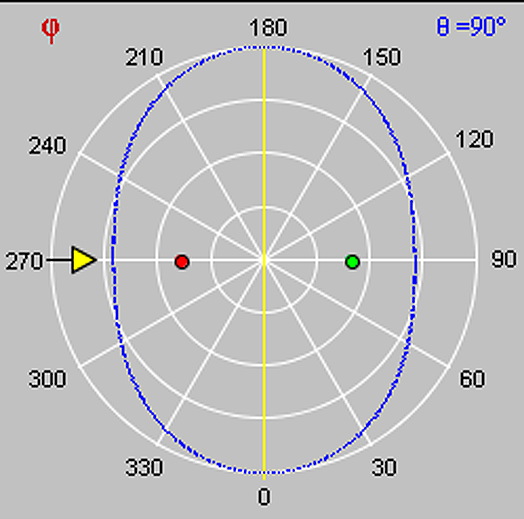
\includegraphics[scale=0.25]{archivos/array/numero/1a} & 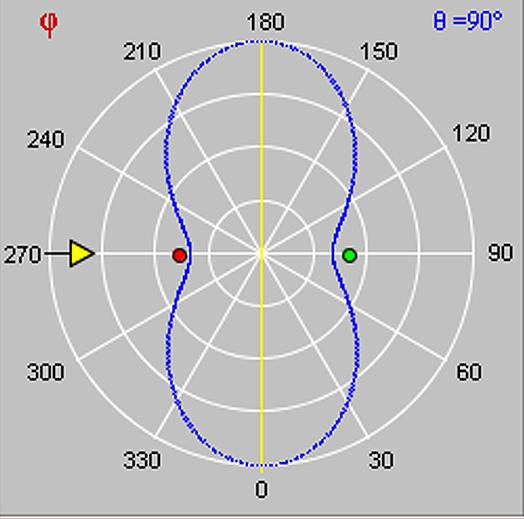
\includegraphics[scale=0.25]{archivos/array/numero/1b} & 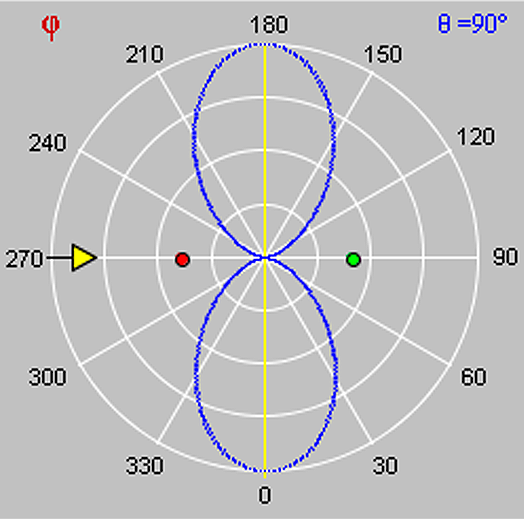
\includegraphics[scale=0.25]{archivos/array/numero/1c} \\
$d=\lambda/4 \; ; \; N=1$  & 
$d=\lambda/4 \; ; \; N=2$  & 
$d=\lambda/4 \; ; \; N=3$  \\

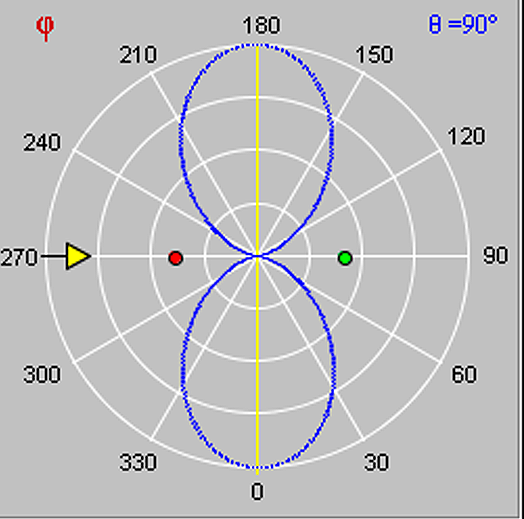
\includegraphics[scale=0.25]{archivos/array/numero/2a} & 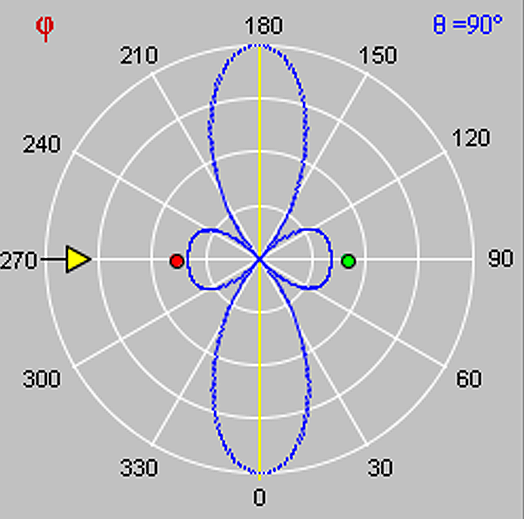
\includegraphics[scale=0.25]{archivos/array/numero/2b} & 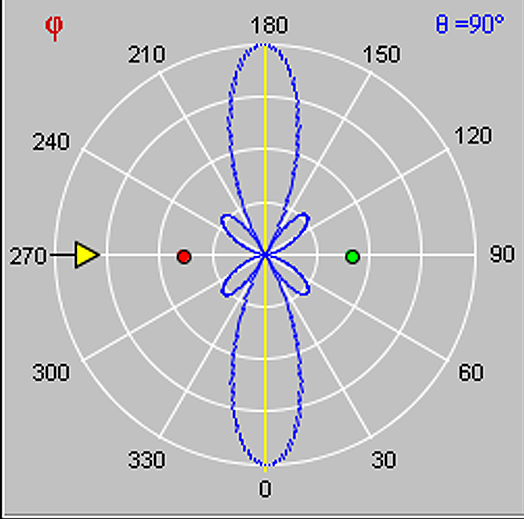
\includegraphics[scale=0.25]{archivos/array/numero/2c} \\
$d=\lambda/2 \; ; \; N=1$  & 
$d=\lambda/2 \; ; \; N=2$  & 
$d=\lambda/2 \; ; \; N=3$  \\

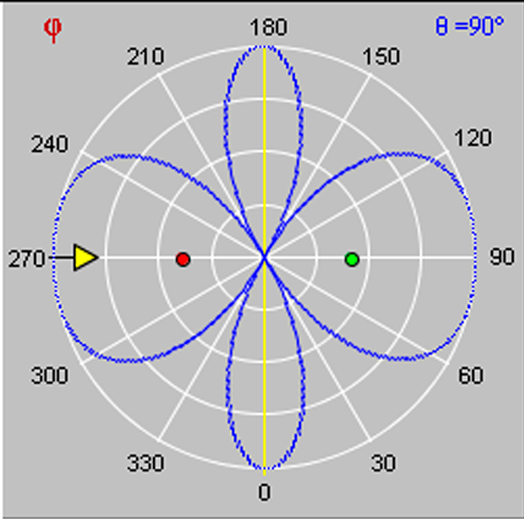
\includegraphics[scale=0.25]{archivos/array/numero/3a} & 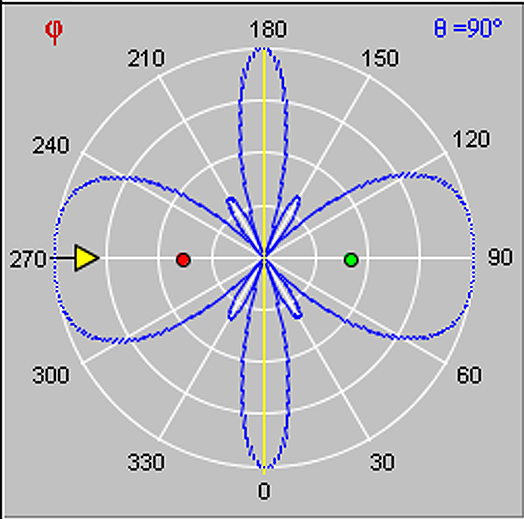
\includegraphics[scale=0.25]{archivos/array/numero/3b} & \includegraphics[scale=0.25]{archivos/array/numero/3c} \\
$d=\lambda \; ; \; N=1$  & 
$d=\lambda \; ; \; N=2$  & 
$d=\lambda \; ; \; N=3$  \\
\end{tabular}
\caption{Efecto de adición de elementos sobre array lineal}
\label{tab:numeroelementos} % 
\end{table}




\subsection{Espaciado de elementos}
\par En esta caso se modificará la separación entre antenas fijando el número de elementos que componen el array a 4 dipolos $\lambda/2$ 

\begin{table}[h]
\centering
\begin{tabular}{ccc}
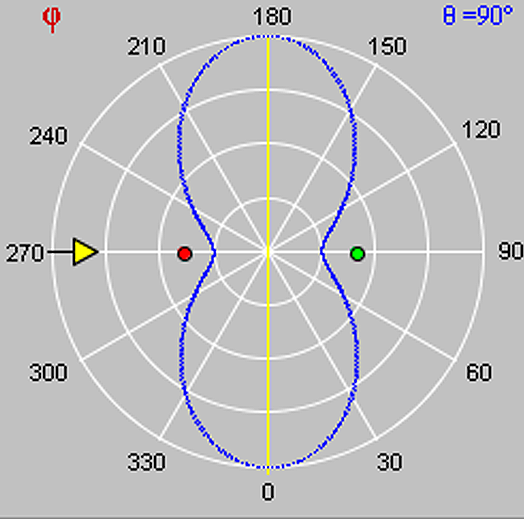
\includegraphics[scale=0.25]{archivos/array/distancia/1a} & 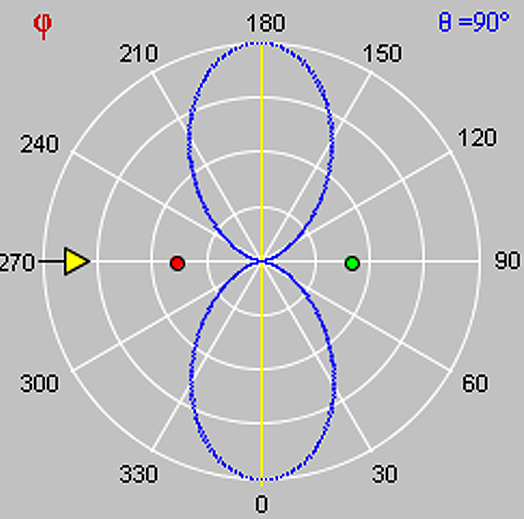
\includegraphics[scale=0.25]{archivos/array/distancia/1b} & 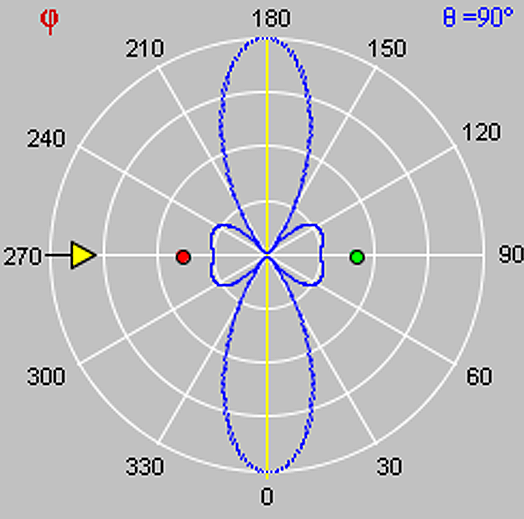
\includegraphics[scale=0.25]{archivos/array/distancia/1c} \\
$d=0.2\lambda$  & 
$d=0.25\lambda$  & 
$d=0.3\lambda$  \\

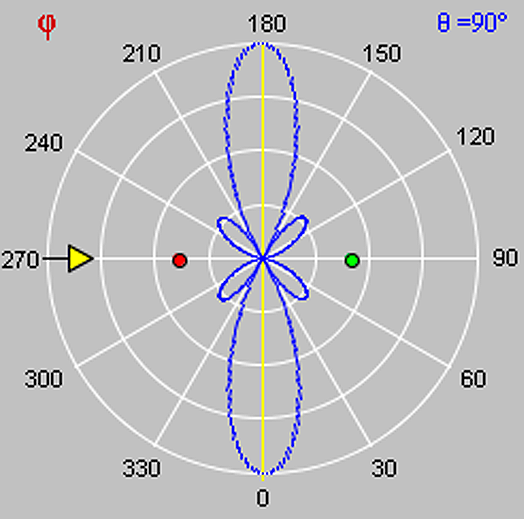
\includegraphics[scale=0.25]{archivos/array/distancia/2a} & 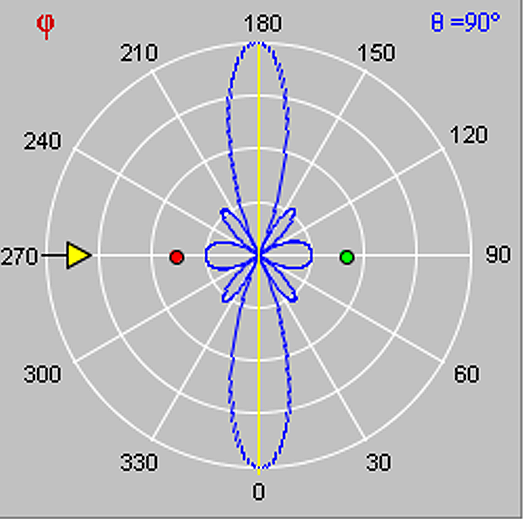
\includegraphics[scale=0.25]{archivos/array/distancia/2b} & 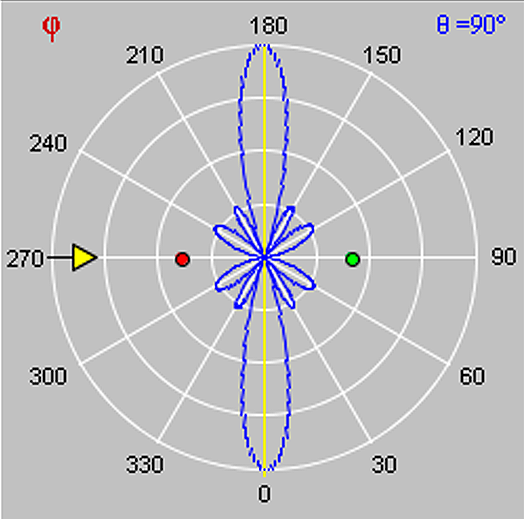
\includegraphics[scale=0.25]{archivos/array/distancia/2c} \\
$d=0.4\lambda$  & 
$d=0.5\lambda$  & 
$d=0.6\lambda$  \\

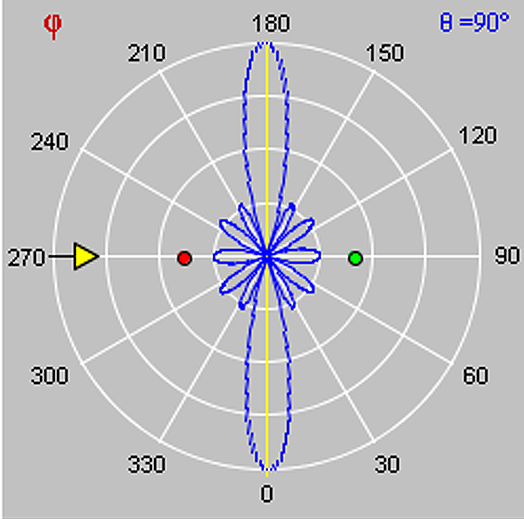
\includegraphics[scale=0.25]{archivos/array/distancia/3a} & 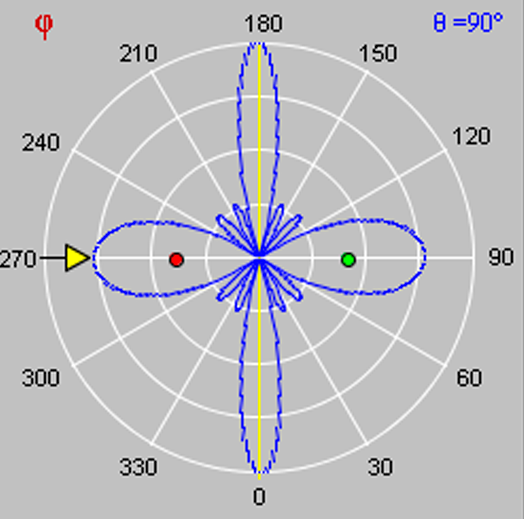
\includegraphics[scale=0.25]{archivos/array/distancia/3b} & \includegraphics[scale=0.25]{archivos/array/distancia/3c} \\
$d=0.75\lambda$  & 
$d=0.8\lambda$  & 
$d=0.9\lambda$  \\
\end{tabular}
\caption{Efecto de la separación de elementos sobre array lineal}
\label{tab:distanciaelementos} % 
\end{table}